\chapter{Metode statistice}

\section{Eliminarea trendului}
\subsection{Metoda regresiei polinomiale}

\noindent Metoda constă în presupunerea că trendul seriei este un polinom de grad mic (2, 3, 4, 5) și calcularea polinomului de regresie. Pașii metodei sunt:\\

\noindent 1) Se consideră valorile seriei de timp $v = [v_0, v_1, ..., v_{n-1}]^T$ și momentele de timp $t = [t_0, t_1, ..., t_{n-1}]^T$ 
la care au fost înregistrate valorile $v$. \\

\noindent 2) Se determină trendul seriei sub forma unui polinom $P$ de grad mic $d$ $\in$ \{2, 3, 4, 5\} prin rezolvarea sistemului liniar $P(t_i)=v_i, 
i \in \{0, 1, ..., n-1\}$ în sensul celor mai mici pătrate. \\ \\
\noindent 3) Seria fără trend este $r = [r_0, r_1, ..., r_{n-1}]^T$, $r_i = v_i - P(t_i)$.\\
\\

\subsection{Metoda regresiei polinomiale - rezolvarea sistemului}
\noindent 1) Polinomul $P$ este reprezentat prin vectorul de coeficienți $c = [c_0, c_1, ..., c_d]^T$, $P = c_0 + c_1X + ... + c_dX^d$.\\

\noindent 2) Matricea sistemului este $A \in M_{n,d+1}(\mathbb{R})$, $A_{i,j} = t_i^j$, $i \in \{0, 1, ..., n-1\}$, $j \in \{0, 1, ..., d\}$.\\

\noindent 3) În ipoteza $n-1$ > $d$ (seria de timp este lungă, iar gradul polinomului este mic), matricea $A$ are rang $d+1$ și sistemul $Ac = v$ admite soluție unică în sensul celor mai mici pătrate ($c$ minimizează norma vectorului $v-Ab$, unde $b$ este un vector din $\mathbb{R}^{d+1}$).\\

\noindent 4) $c = (A^TA)^{-1}A^Tv$.

\section{Detectarea anomaliilor}

\subsection{Metoda z-score}
\noindent Ideea metodei constă în presupunerea că valorile din seria fără trend reprezintă eșantioane dintr-o distributie normală de medie $m$ 
și deviație standard $sd$. Apoi se calculează estimatorii de verosimilitate maximă \cite{normal_mle}, în acest caz media empirică pentru medie 
și varianța empirică pentru pătratul deviației standard. Pașii metodei sunt:\\

\noindent 1) Se lucrează pe serii fără trend $r = [r_0, r_1, ..., r_{n-1}]^T$.\\

\noindent 2) Se calculează media $m = \frac{1}{n}\sum\limits_{i=0}^{n-1}r_i$ și deviația standard $sd = \sqrt{\frac{1}{n}\sum\limits_{i=0}^{n-1}(r_i-m)^2}$.\\

\noindent 3) Se calculează $z = [z_0, z_1, ..., z_{n-1}]^T$, $z_i = \frac{1}{sd}(r_i-m)$.\\

\noindent 4) Se consideră anomalii valorile $z_i$ cu modulul mai mare decât un anumt prag (de obicei 2 sau 3 sau chiar și mai mic).

\subsection{Metoda medie mobilă}
\noindent Ideea metodei constă în calcularea mediei pe o fereastră glisantă, în loc de toată seria, în scopul de a neglija posibile oscilații 
ale seriei. Pașii metodei sunt:\\

\noindent 1) Se lucrează pe serii fără trend $r = [r_0, r_1, ..., r_{n-1}]^T$.\\

\noindent 2) Se calculează media mobilă pe fiecare fereastră glisantă de lungime $ws$, cu pas $step < ws$.\\

\noindent 3) După ce se calculează diferența față de medie pe toate ferestrele, valorile care depășesc un anumit prag sunt considerate anomalii.

\subsection{Metoda de deviație medie absolută}
\noindent Ideea metodei constă în presupunerea că valorile din seria fără trend reprezintă eșantioane dintr-o distributie Laplace de parametri $m$ 
și $s$. Apoi se calculează estimatorii de verosimilitate maximă \cite{laplace_mle}, în acest caz mediana empirică pentru $m$ 
și deviația absolută medie pentru $s$. \\ 

\noindent Pașii metodei sunt:\\

\noindent 1) Se lucrează pe serii fără trend $r = [r_0, r_1, ..., r_{n-1}]^T$.\\

\noindent 2) Se calculează mediana seriei de timp. Mediana ($p$) este o valoare aleasă astfel încât jumătate din valori să fie $\ge p$ și jumătate din valori să 
fie $\le p$ (în practică vom alege mijlocul vectorului sortat).\\

\noindent 3) Se calculează deviația absolută medie $s = \frac{1}{n}\sum\limits_{i=0}^{n-1}|r_i-p|$.\\

\noindent 4) Se calculează $z = [z_0, z_1, ..., z_{n-1}]^T$, $z_i = \frac{1}{s}(r_i-p)$.\\

\noindent 5) Se consideră anomalii valorile $z_i$ cu modulul mai mare decât un anumt prag.

\subsection{Metoda procentuală}
\noindent Presupunem că apar anomalii pe un anumit procent (cunoscut) din serie (de exemplu, procent aproximat de o metodă Fourier). 
Se aplică una dintre metodele anterioare cu diferența că pragul se ajustează pentru a obține procentul dorit de anomalii.

\section{Alegerea pragurilor}

\noindent Pentru calcularea pragurilor pentru fiecare metodă se folosește metoda procentuală. Folosind seria fără trend 
$r = [r_0, r_1, ..., r_{n-1}]^T$, verificăm ce amplitudine au frecvențele 3, 4 și 5 (frecvențele 0, 1 și 2 reprezintă eventuale componente ale 
trendului ce nu au fost eliminate, iar frecvențele mai mari decât 5 reprezintă sezonalitatea și zgomotul). Implementare:\\

\noindent 1) Se lucrează cu serii fără trend $r = [r_0, r_1, ..., r_{n-1}]^T$.\\

\noindent 2) Se calculează transformata Fourier a seriei $z = [z_0, z_1, ..., z_{n-1}]^T$.\\

\noindent 3) Se calculează suma amplitudinilor frecvențelor 3, 4, 5 (care pot indica anomalii).\\

\noindent 4) Dacă una dintre aceste frecvențe este frecvența de amplitudine maximă, se neglijează 
(reprezintă probabil o componentă importantă a sezonalității).\\

\noindent 5) Se împarte suma obținută la suma tuturor frecvențelor. Această valoare va fi folosită ca $procent$ de anomalii.\\

\noindent 6) Se caută pragul optim pentru fiecare metodă în parte. Se stabilește limita inferioară a pragului la 1. Apoi se folosește observația că numărul de 
anomalii scade cu creșterea pragului ($anomalii(prag)$ este o funcție descrescătoare). Se pornește cu limita superioară a pragului setată la 2 și 
această limită se tot dublează cât timp dă procent de anomalii mai mare decât $procent$. În final se caută pragul optim între limita inferioară (=1) 
și limita superioară prin metoda bisecției.

\section{Concluzii}
\noindent Metodele statistice se dovedesc a fi în același timp simple și eficiente la detectarea anomaliilor când se lucrează cu seria generală, așa 
cum se vede din testarea lor pe un set de date. Din punct de vedere al timpului de execuție, complexitățile algoritmilor sunt: O($n$) pentru 
determinarea trendului, O($n$) pentru z-score și medie mobilă, O($n$log$n$) pentru deviație absolută, O($n$log$n$) pentru determinarea procentului în 
cazul metodei procentuale. Căutarea efectivă a pragului are aceeași clasă de complexitate ca metoda pentru care se caută pragul. \\

\noindent Imaginea de mai jos exemplifică rularea metodei deviației absolute cu prag determinat automat pe un set de date despre prețurile a 6 categorii de acțiuni.\\
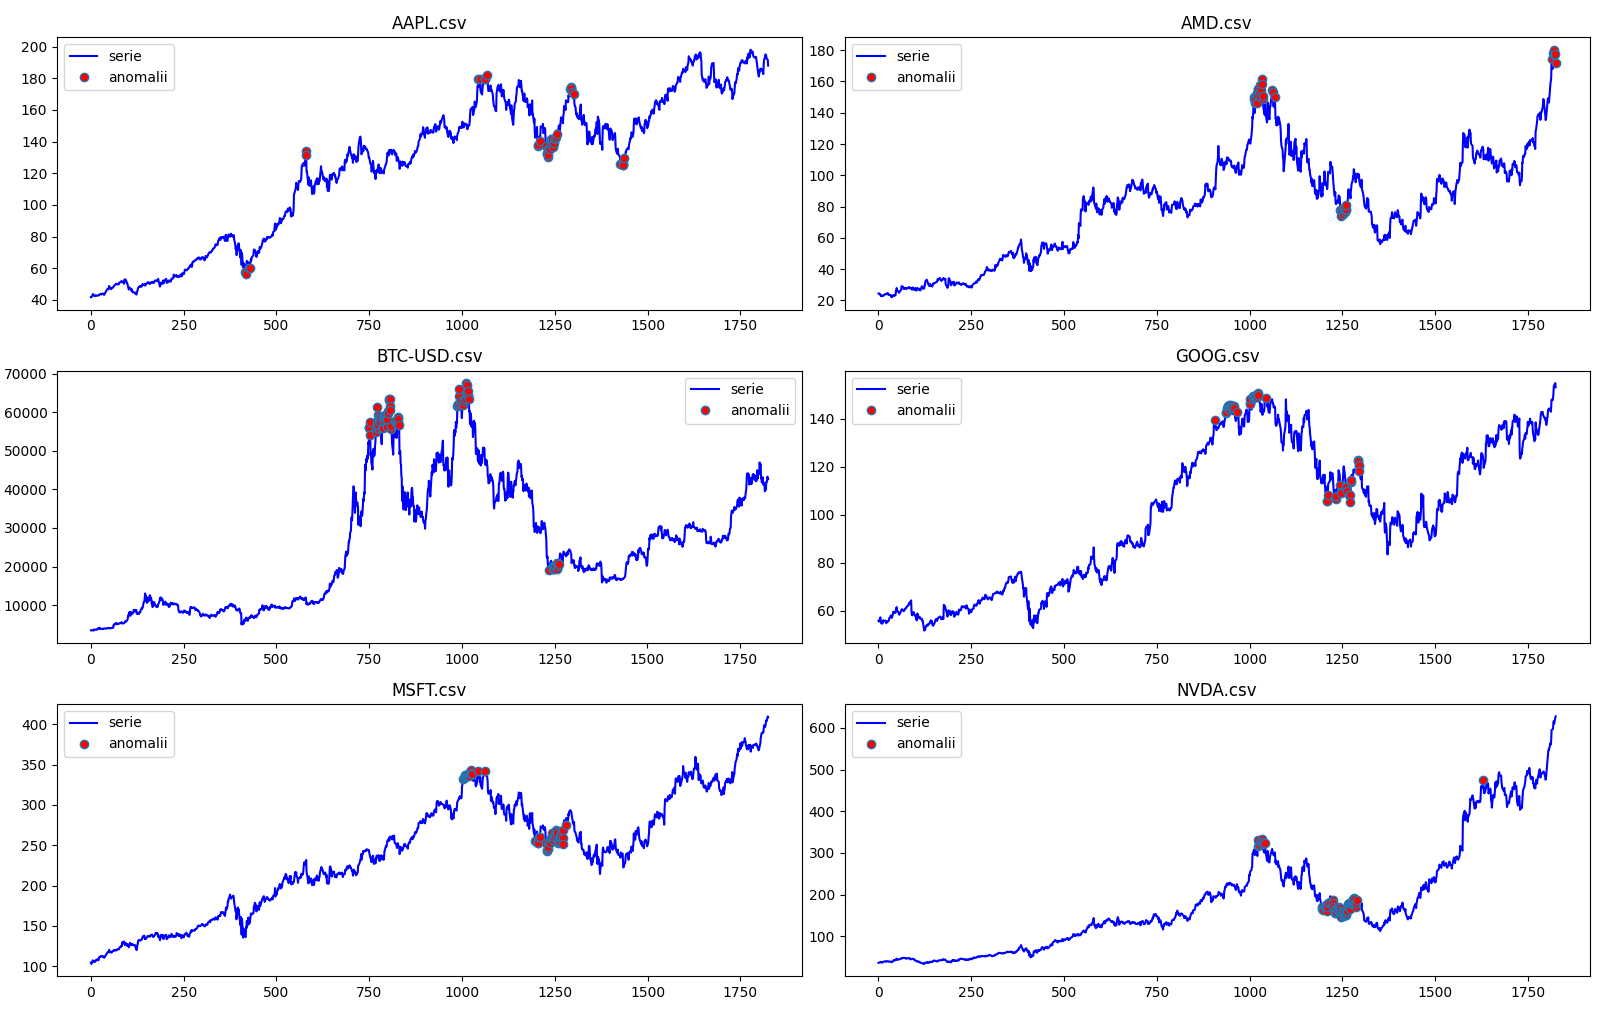
\includegraphics[width=\linewidth]{deviatie_absoluta.png}

%\chapter{Detectarea anomaliilor în ultimul punct al seriei}
%TBD